% This document is based on a template created by Ted Pavlic (http://www.tedpavlic.com)


%----------------------------------------------------------------------------------------
%	PACKAGES AND OTHER DOCUMENT CONFIGURATIONS
%----------------------------------------------------------------------------------------

\documentclass{article}

\usepackage{fancyhdr} % Required for custom headers
\usepackage{lastpage} % Required to determine the last page for the footer
\usepackage{extramarks} % Required for headers and footers
\usepackage[usenames,dvipsnames]{color} % Required for custom colors
\usepackage{graphicx} % Required to insert images
\usepackage{subcaption}
\usepackage{listings} % Required for insertion of code
\usepackage{courier} % Required for the courier font
%\usepackage{lipsum} % Used for inserting dummy 'Lorem ipsum' text into the template
\usepackage{amsmath,physics,siunitx,amssymb}
\usepackage{placeins}
\usepackage[backend=biber,style=ieee]{biblatex}
\usepackage{enumitem}
\usepackage{hyperref,cleveref}

\addbibresource{fakebonus.bib}

% Margins
\topmargin=-0.45in
\evensidemargin=0in
\oddsidemargin=0in
\textwidth=6.5in
\textheight=9.0in
\headsep=0.25in

\linespread{1.1} % Line spacing

% Set up the header and footer
\pagestyle{fancy}
\lhead{\hmwkAuthorName} % Top left header
\chead{\hmwkClass\ (\hmwkClassTime): \hmwkTitle} % Top center head
%\rhead{\firstxmark} % Top right header
\lfoot{\lastxmark} % Bottom left footer
\cfoot{} % Bottom center footer
\rfoot{Page\ \thepage\ of\ \protect\pageref{LastPage}} % Bottom right footer
\renewcommand\headrulewidth{0.4pt} % Size of the header rule
\renewcommand\footrulewidth{0.4pt} % Size of the footer rule

\DeclareMathOperator*{\argmax}{arg\,max}

%\setlength\parindent{0pt} % Removes all indentation from paragraphs

%----------------------------------------------------------------------------------------
%	DOCUMENT STRUCTURE COMMANDS
%	Skip this unless you know what you're doing
%----------------------------------------------------------------------------------------

% Header and footer for when a page split occurs within a problem environment
\newcommand{\enterproblemHeader}[1]{
%\nobreak\extramarks{#1}{#1 continued on next page\ldots}\nobreak
%\nobreak\extramarks{#1 (continued)}{#1 continued on next page\ldots}\nobreak
}

% Header and footer for when a page split occurs between problem environments
\newcommand{\exitproblemHeader}[1]{
%\nobreak\extramarks{#1 (continued)}{#1 continued on next page\ldots}\nobreak
%\nobreak\extramarks{#1}{}\nobreak
}

\setcounter{secnumdepth}{0} % Removes default section numbers
\newcounter{problem} % Creates a counter to keep track of the number of problems
\setcounter{problem}{-1}

\newcommand{\problemName}{}
\newenvironment{problem}[1][Part \theproblem]{ % Makes a new environment called problem which takes 1 argument (custom name) but the default is "problem #"
	\stepcounter{problem} % Increase counter for number of problems
	\renewcommand{\problemName}{#1} % Assign \problemName the name of the problem
	\section{\problemName} % Make a section in the document with the custom problem count
	\enterproblemHeader{\problemName} % Header and footer within the environment
}{
	\exitproblemHeader{\problemName} % Header and footer after the environment
}

\newcommand{\problemAnswer}[1]{ % Defines the problem answer command with the content as the only argument
	\noindent\framebox[\columnwidth][c]{\begin{minipage}{0.98\columnwidth}#1\end{minipage}} % Makes the box around the problem answer and puts the content inside
}

\newcounter{subproblem}[problem]
\newcommand{\subproblemName}{}
\newenvironment{subproblem}[1][\theproblem~(\alph{subproblem})]{ % New environment for sections within  problems, takes 1 argument - the name of the section
	\stepcounter{subproblem}
	\renewcommand{\subproblemName}{#1} % Assign \problemName the name of the problem
	\subsection{\subproblemName} % Make a section in the document with the custom problem count
	\enterproblemHeader{\subproblemName} % Header and footer within the environment
}{
	\enterproblemHeader{\problemName} % Header and footer after the environment
}

\newcommand{\numberthis}{\addtocounter{equation}{1}\tag{\theequation}}

%----------------------------------------------------------------------------------------
%	NAME AND CLASS SECTION
%----------------------------------------------------------------------------------------

\newcommand{\hmwkTitle}{Assignment\ \#$3$} % Assignment title
\newcommand{\hmwkDueDate}{Monday,\ March\ 19,\ 2018} % Due date
\newcommand{\hmwkClass}{CSC411} % Course/class
\newcommand{\hmwkClassTime}{L2001} % Class/lecture time
\newcommand{\hmwkAuthorName}{Lukas Zhornyak} % Your name

%----------------------------------------------------------------------------------------
%	TITLE PAGE
%----------------------------------------------------------------------------------------

\title{
	\vspace{2in}
	\textmd{\textbf{\hmwkClass:\ \hmwkTitle}}\\
	\normalsize\vspace{0.1in}\small{Due\ on\ \hmwkDueDate}\\
	\vspace{0.1in}
	\vspace{3in}
}

\author{\textbf{\hmwkAuthorName}}
%\date{} % Insert date here if you want it to appear below your name

%----------------------------------------------------------------------------------------

\begin{document}

\maketitle
\clearpage

%----------------------------------------------------------------------------------------
%	ENVIRONMENT
%----------------------------------------------------------------------------------------

\begin{problem}[Environment]	
	Parts 1-6 were created with Python 2.7.14 with numpy 1.14.0, scipy 1.0.0, scikit-image 0.13.1, and matplotlib 2.1.1, as well as all associated dependencies. 
\end{problem}
\clearpage

%----------------------------------------------------------------------------------------
%	PART 1
%----------------------------------------------------------------------------------------
\FloatBarrier
\begin{problem}
	
	\begin{subproblem}
		To improve on the performance of the models previously tested, a convolutional neural network is used, based closely on the model presented in \cite{DBLP:journals/corr/Kim14f}. In summary, this network has multiple one dimensional convolution layers of different filter sizes acting on the input vectors. The maximum activation of these filters across the entire sentence are then combined in a final fully-connected layer. The data is presented to the neural network in a slightly different manner than it was to the previous models, consisting of several vectors each representing one word rather than one vector representing all the words. In this way, the network is able to additional, positional information relating to the headlines. 
		
		The various hyperparameters used in the model were those found to be most effective in the original study. Three sizes of filters were used (three, four and five words), each with one hundred filters. Early stopping was employed, so training ended after performance on the validation set did not improve for two epochs. Additionally, the length of a sentence was cut off after forty words owing to memory and performance constraints. As the large majority of headlines have fewer than forty words, this is not expected to reduce performance significantly. The model was trained using stochastic gradient descent with a learning rate of \num{e-4}.
		
		The model was trained on the original dataset presented. The learning curve associated with this training is shown in \cref{learning}. The final accuracy achieved was 96.24\% on the training set, but only 69.38\% on the validation set and 68.57\%.  While the accuracy on the training set is comparable to those of other models, the performance on the other sets is much worse, suggesting a large degree of overfitting and that the relations that the model uses to classify a sentence are not effective for the task of fake new detection.
		
		Additional tests were performed by training the model on the "Liar" dataset \cite{DBLP:journals/corr/Wang17j}. In this set, statements labelled "true", "mostly-true", or "half-true" were considered to represent real news, while other labels signified fake news. The performance in this dataset is similar, albeit worse, to that observed in the previous, achieving 92.38\% on the training set, 58.41\% on the validation set, and 59.51\% on the testing set. However, the model trained on this set performed worse than chance on the original data set, achieving 44.66\% accuracy. This suggests that, on top of not being very effective in the first place, this framework in this context does not produce easily transferable models. For this reason, the model trained on the original data set is used for all further purposes.
		
		\begin{figure}
			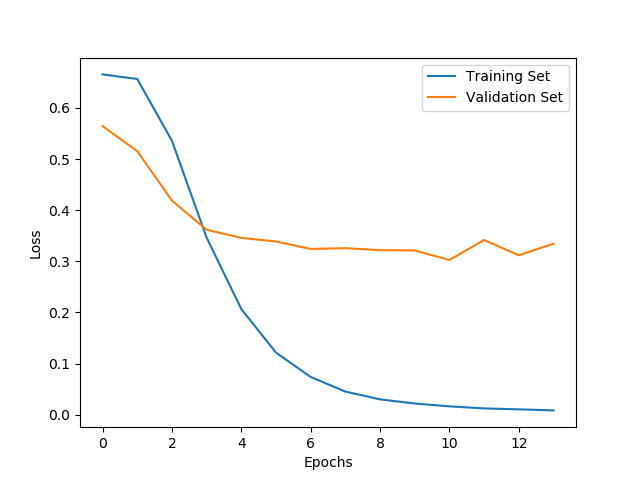
\includegraphics[width=\linewidth]{error_orig}
			\caption{Learning curve for the training and validation sets across epochs. Early stopping was employed, so training ended after performance on the validation set did not improve for two epochs.}
			\label{learning}
		\end{figure}
	\end{subproblem}

	\begin{subproblem}
		Since this model examines sequences of words rather than individual words, finding the top words in this context does not have much meaning. Instead, the sequence of words that most activate the filter that has the largest corresponding weight in the fully connected layer are generated. These are listed in .... These sequences do not seem to form coherent phrases, nor do they share very many words with those were identified for previous model.
		\begin{table}
			\begin{tabular}{cc}
				Real Sequences & Fake sequences \\
				cia chickens tumultuous stir debuts & suddenly silicon message everywhere \\ 
				analysis contradicts fashion opinion & pena sound follows includes \\
				tradition load liberals cares & watch that m \\
				trumps australia talks & shredded revolt slams thinks mired \\
				labels democrats website coy & homeless hillary america \\
				trumps australia ban & just an trump \\
				killed adjusted responds promoting & road henderson military annouces hurricanes \\
				hallways judges with gore & voting just that \\
				thrilled exporters softens antique ability & painter punish off inevitable \\
				preemptive guidelines spending repartis refugee & sack duke aware request marblenecltr
			\end{tabular}
		\end{table}
	\end{subproblem}
	
\end{problem}
\clearpage

%----------------------------------------------------------------------------------------

\printbibliography

\end{document}